\documentclass[12pt, a4paper]{article}

% ── 1. GÓI LỆNH CƠ BẢN ────────────────────────────────────────────────────────
\usepackage[utf8]{inputenc}
\usepackage[T1]{fontenc}
\usepackage[vietnamese,english]{babel}
\usepackage[a4paper, margin=2.5cm]{geometry}
\usepackage{graphicx} 
\usepackage{tikz}     
\usetikzlibrary{calc}
\usepackage{setspace}
\usepackage{parskip}
\usepackage{amsmath, amssymb}
\usepackage{booktabs}
\usepackage{enumitem}
\usepackage{xcolor}
\usepackage{listings}  
\usepackage{fancyhdr}  
\usepackage{titlesec}
\usepackage[round]{natbib} % QUAN TRỌNG: Gói lệnh bắt buộc cho \citep và \citet
\usepackage{hyperref}
\usepackage{float}
\usepackage{caption}

% ── 2. HEADER/FOOTER ─────────────────────────────────────────────────────────
\pagestyle{fancy}
\fancyhf{} 
\fancyhead[L]{\footnotesize\color{gray}Group 13 -- DSEB 66A}
\fancyfoot[R]{\footnotesize Page \thepage}
\renewcommand{\headrulewidth}{0.4pt}

% ── 3. ĐỊNH DẠNG CODE (LISTINGS) ─────────────────────────────────────────────
\definecolor{codegreen}{rgb}{0,0.6,0}
\definecolor{backcolour}{rgb}{0.95,0.95,0.92}
\lstset{
    backgroundcolor=\color{backcolour},
    commentstyle=\color{codegreen},
    basicstyle=\ttfamily\footnotesize,
    breaklines=true,
    breakatwhitespace=false,
    columns=fullflexible,
    keepspaces=true,
    frame=single
}

% ── 4. ĐỊNH DẠNG TIÊU ĐỀ (SECTION) ──────────────────────────────────────────
\definecolor{darkblue}{RGB}{31, 78, 121}
\titleformat{\section}{\large\bfseries\color{darkblue}}{\thesection}{1em}{}
\titleformat{\subsection}{\normalsize\bfseries\color{darkblue}}{\thesubsection}{1em}{}

% ── BẮT ĐẦU NỘI DUNG ─────────────────────────────────────────────────────────
\begin{document}
\pagenumbering{gobble}

% =============== TRANG BÌA ===============
\begin{titlepage}
\thispagestyle{empty}
\begin{tikzpicture}[remember picture, overlay]
  % Logo mờ ở giữa
  \node[inner sep=0pt, opacity=0.08] at (current page.center) {
    \includegraphics[width=1.2\paperwidth]{logo_neu.png}
  };
  
  % Khung nội dung chính
  \node[draw=black, very thick, rounded corners=10pt,
        inner xsep=1.5em, inner ysep=1.5em, text width=\textwidth,
        align=center, fill=white, opacity=0.98] at (current page.center) {
    \begin{minipage}{\textwidth}
      \centering
      {\Large \textbf{NATIONAL ECONOMICS UNIVERSITY}} \\
      {\large \textbf{FACULTY OF MATHEMATICAL ECONOMICS}}\vspace{1.5em}
      
      \includegraphics[width=0.3\linewidth]{logo_neu.png}\vspace{1.5em}
      
      {\large \textbf{GROUP 13}} \\
      {\large \textbf{ECONOMETRICS GROUP PROJECT}}\vspace{2em}

      {\LARGE \textbf{Wage Determinants and Human Capital: An Econometric Analysis}}\vspace{0.8em}
      
      {\large Evidence from a Cross-Sectional Employee Dataset}\vspace{3em}
      
      \begin{flushleft}
      \hspace{4em}\textbf{Course:} Econometrics \\
      \hspace{4em}\textbf{Lecturers:} Mr. Nguyen Manh The \\
      \hspace{9.4em} Ms. Nguyen Thi Thuy Trang \\
      \hspace{4em}\textbf{Class:} DSEB 66A \\
      \hspace{4em}\textbf{Team members:} Lai Minh An - 11245829 \\
      \hspace{10.8em} Nguyen Minh Duc - 11245859 \\
      \hspace{10.8em} Bui Duc Duy - 11245867 \\
      \hspace{10.8em} Nguyen Manh Duy - [Insert ID]
      \end{flushleft}
      \vspace{2.5em}
      
      \textbf{HANOI, 2026}
    \end{minipage}
  };
\end{tikzpicture}
\end{titlepage}

\clearpage
\pagenumbering{arabic}
\setcounter{page}{1}

% =============== MỤC LỤC ===============
\onehalfspacing
\tableofcontents
\newpage

% =============== NỘI DUNG ===============
\section{Introduction of the Research}

The primary objective of this research is to empirically quantify the impacts of key
human capital determinants — namely \textit{Age}, \textit{Gender}, \textit{Education Level},
and \textit{Years of Experience} — on individual salary levels. In the context of a rapidly
evolving labour market, understanding these drivers is crucial for identifying wage
determination patterns and potential systemic disparities such as the gender pay gap.

% ── 1.1 ───────────────────────────────────────────────────────────────────────
\subsection{Research Gap and Motivation}

While a substantial body of literature has examined the determinants of wages in
developed economies \citep{mincer1974, card1999, lemieux2006}, empirical evidence drawn
from smaller, cross-sectional professional datasets remains comparatively sparse.
Existing studies tend to rely on large-scale administrative records or national labour
force surveys, which may obscure the dynamics present in specific professional labour
market segments. This study contributes to the literature by offering a focused,
micro-level empirical analysis, providing estimates of returns to human capital that are
directly applicable to professional labour market contexts.

Moreover, the explicit modelling of non-linear age effects and education--experience
interactions — rarely examined jointly in smaller samples — represents a methodological
contribution that addresses limitations in prior cross-sectional studies.

% ── 1.2 ───────────────────────────────────────────────────────────────────────
\subsection{Data Description and Outlier Treatment}

The analysis utilises a cleaned dataset drawn from an initial raw sample of 669 observations. Prior to analysis, a systematic data auditing procedure was conducted in two stages to ensure data quality and the validity of subsequent statistical inference.

In the first stage, duplicate records --- defined as observations sharing identical values across all key variables (\textit{Age, Gender, Education Level, Years of Experience, and Salary}) --- were identified and removed. Their retention would artificially inflate the effective sample size, introduce non-random repetition into the error structure, and violate the OLS assumption of independently distributed observations \citep{wooldridge2010}. Following deduplication, 426 unique observations were retained. Key variables include \textit{age} (in years), \textit{gender} (binary: male/female), \textit{highest educational qualification}, \textit{years of professional experience}, and \textit{annual gross salary} (in USD).

In the second stage, the diagnostic phase identified a significant extreme outlier ($ \text{Salary} = \$350 $) using a hybrid detection rule combining the Interquartile Range (IQR) method and a log-modified Z-score criterion. This observation was flagged as implausible given the broader salary distribution and the professional nature of the sample. To further ensure the robustness of estimated coefficients, this outlier was excluded, yielding a final analytical sample of \textbf{$ n = 425 $} observations.

% ── 1.3 ───────────────────────────────────────────────────────────────────────
\subsection{Scope and Limitations}

It is acknowledged that a sample of $n = 425$ observations constitutes a limitation on
the generalisability of findings, particularly when estimating interaction effects and
higher-order polynomial terms (Model~3). Accordingly, results should be interpreted as
indicative of directional relationships rather than precise population-level estimates.
Future research should seek to replicate these findings using larger, probability-sampled
datasets.

% ══════════════════════════════════════════════════════════════════════════════
\section{Theoretical Background and Methods}

This research is theoretically grounded in the \textbf{Human Capital Theory}
\citep{becker1964}, which posits that individuals invest in education and vocational
training to enhance their marginal productivity, which is subsequently rewarded by higher
market wages. The theory treats education and experience not as consumption goods but as
investments yielding measurable returns in the form of increased earnings over the life
cycle.

% ── 2.1 ───────────────────────────────────────────────────────────────────────
\subsection{The Mincer Wage Equation}

To operationalise this theory, we employ the \textbf{Mincer Wage Equation}
\citep{mincer1974}, a cornerstone of labour economics that models earnings as a function
of schooling and work experience. The semi-logarithmic functional form is preferred
because it:
\begin{enumerate}[label=(\roman*), leftmargin=2em]
  \item allows regression coefficients to be interpreted as approximate percentage
        returns to investments in human capital;
  \item accommodates the right-skewed nature of wage distributions; and
  \item typically mitigates non-constant variance (heteroscedasticity) in wage regressions, as discussed by \citet{wooldridge2010}, though the effectiveness of this transformation varies across datasets and residual heteroskedasticity may persist depending on the underlying variance structure.
\end{enumerate}

The general Mincerian form is expressed as:

\begin{equation}
  \ln(\text{Salary}_i) = \beta_0 + \beta_1\,\text{Education}_i
    + \beta_2\,\text{Experience}_i
    + \beta_3\,\text{Experience}_i^2
    + u_i
  \label{eq:mincer}
\end{equation}

% ── 2.2 ───────────────────────────────────────────────────────────────────────
\subsection{Model Adaptations and Variable Definitions}

In this research, the Mincerian framework (Equation~\ref{eq:mincer}) is extended to
incorporate additional human capital and demographic controls:

\begin{itemize}[leftmargin=1.5em]
  \item \textbf{Education:} Captured via dummy variables for attainment levels —
        Bachelor's Degree, Master's Degree, and PhD — with \textit{High School} as the
        reference (base) category. This specification allows for non-linear,
        level-specific returns to schooling.

  \item \textbf{Experience:} Measured in years of continuous professional work
        experience. In Model~3, a quadratic term
        ($\text{Experience}^2$) is included to capture potential diminishing returns.

  \item \textbf{Age:} Included to capture life-cycle earnings dynamics and potential
        labour market entry/exit effects. Age is mean-centred
        ($\text{Age}_c = \text{Age} - \overline{\text{Age}}$) in Model~3 to mitigate
        structural multicollinearity with Experience (see Section~2.3).

  \item \textbf{Gender:} A binary dummy variable ($1 = \text{Male}$,
        $0 = \text{Female}$) included as a control to investigate gender-based wage
        differentials, consistent with the equal pay literature \citep{blaukahn2017}.
\end{itemize}

% ── 2.3 ───────────────────────────────────────────────────────────────────────
\subsection{Multicollinearity Between Age and Experience}

A critical methodological concern in wage equations that include both \textit{Age} and
\textit{Experience} is the high degree of structural collinearity between the two
variables. In most professional datasets:
\[
  \text{Age} \approx \text{Education Duration} + \text{Experience} + \text{Entry Age}
\]
implying that Age and Experience are structurally correlated. When both are entered in
their raw form into the same OLS regression, the Variance Inflation Factor (VIF) for
these variables may exceed conventional thresholds ($\text{VIF} > 10$), rendering
individual coefficient estimates unstable and difficult to interpret.

Unlike studies that exclude Age entirely due to multicollinearity with Experience, this study retains Age to capture life-cycle earnings effects that are theoretically distinct from accumulated work experience. Specifically, Age reflects broader labour market dynamics — including cohort effects, career interruptions, and seniority norms — that Experience alone cannot fully proxy. Variable exclusion, while parsimonious, risks omitted variable bias if Age exerts an independent effect on salary conditional on Experience. Accordingly, this study addresses the collinearity concern through mean-centring rather than exclusion.

To address this, Model~3 employs mean-centred age ($\text{Age}_c$) and its quadratic
term ($\text{Age}_c^2$). Centring removes the structural component of multicollinearity
by shifting the origin of the age variable to its sample mean, while preserving the
non-linear relationship of interest. Residual multicollinearity will be formally
diagnosed using VIF statistics reported in the results section.

% ══════════════════════════════════════════════════════════════════════════════
\section{Model Specification and Hypotheses}

We specify three nested Ordinary Least Squares (OLS) models to evaluate the stability of
estimates across different functional specifications. The nested structure allows
assessment of whether marginal complexity additions yield statistically and economically
meaningful improvements in model fit.

% ── 3.1 ───────────────────────────────────────────────────────────────────────
\subsection{Model 1 — Level-Level (Baseline)}

A baseline linear model investigating absolute salary changes:

\begin{equation}
  \text{Salary} = \beta_0 + \beta_1\,\text{Age} + \beta_2\,\text{Exp}
    + \beta_3\,\text{Gender}
    + \sum_{j}\gamma_j\,\text{Education}_j + u
  \label{eq:m1}
\end{equation}

This model establishes a benchmark and is interpretable in levels (USD). Its primary
limitation is the assumption of a linear, additive salary structure, which is unlikely to
hold given the well-documented right-skewness of wage distributions.

% ── 3.2 ───────────────────────────────────────────────────────────────────────
\subsection{Model 2 — Log-Level (Primary Specification)}

Our primary specification, examining percentage changes in salary:

\begin{equation}
  \ln(\text{Salary}) = \beta_0 + \beta_1\,\text{Age} + \beta_2\,\text{Exp}
    + \beta_3\,\text{Gender}
    + \sum_{j}\gamma_j\,\text{Education}_j + u
  \label{eq:m2}
\end{equation}

This form typically provides a superior fit for right-skewed wage distributions.
Coefficients on continuous variables are interpreted as semi-elasticities (approximate
\% change in salary per unit increase in the regressor). For dummy variables, the exact
percentage effect is computed as:
\[
  \%\,\text{effect} = \left(e^{\hat{\beta}} - 1\right) \times 100\%
\]

% ── 3.3 ───────────────────────────────────────────────────────────────────────
\subsection{Model 3 — Log-Level Extended (Non-Linear + Interactions)}

Extends Model~2 by incorporating non-linearities in age and conditional returns to
experience by education level:

\begin{equation}
\begin{aligned}
  \ln(\text{Salary}) ={}& \beta_0
    + \beta_1\,\text{Age}_c
    + \beta_2\,\text{Age}_c^2
    + \beta_3\,\text{Exp}
    + \beta_4\,\text{Gender} \\
    &+ \sum_{j}\gamma_j\,\text{Edu}_j
    + \sum_{j}\delta_j\,(\text{Edu}_j \times \text{Exp})
    + u
\end{aligned}
  \label{eq:m3}
\end{equation}

The inclusion of $\text{Age}_c^2$ allows the earnings--age profile to take an inverted
U-shape, consistent with life-cycle human capital theory \citep{benporath1967}. The
interaction terms $(\text{Edu}_j \times \text{Exp})$ allow the marginal return to
experience to differ by education level, directly testing whether higher-educated workers
exhibit steeper earnings trajectories (H4).

% ── 3.4 ───────────────────────────────────────────────────────────────────────
\subsection{Model Selection Criteria}

The three models will be compared using the following criteria:

\begin{itemize}[leftmargin=1.5em]
  \item \textbf{Adjusted $R^2$:} Penalises unnecessary complexity; used to assess
        incremental explanatory power across nested models.
  \item \textbf{AIC and BIC:} Preferred for nested model comparison as they balance
        goodness-of-fit against parameter count.
  \item \textbf{F-test for joint significance:} Applied when comparing nested
        specifications (e.g., Model~2 vs.\ Model~3) to test whether additional terms
        jointly contribute to explanatory power.
  \item \textbf{Diagnostic tests:} Breusch--Pagan test for heteroscedasticity; VIF for
        multicollinearity; Jarque--Bera test for normality of residuals.
\end{itemize}

% ── 3.5 ───────────────────────────────────────────────────────────────────────
\subsection{Base Categories and Research Hypotheses}

The following base categories are defined for all dummy variable specifications:

\begin{itemize}[leftmargin=1.5em]
  \item \textbf{Gender:} Female (coded 0)
  \item \textbf{Education Level:} High School (omitted reference group)
\end{itemize}

Based on Human Capital Theory and prior empirical evidence, the following research hypotheses are formulated and will be tested at the 5\% significance level (\textit{ceteris paribus}):

\begin{itemize}[leftmargin=1.5em]
  \item \textbf{H1: Returns to Experience}
\end{itemize}
$H_0: \beta_{\text{Exp}} = 0$ (Experience has no effect on salary)\\
$H_1: \beta_{\text{Exp}} > 0$ (Experience increases salary)

\begin{itemize}[leftmargin=1.5em]
  \item \textbf{H2: Education Premium} (Reference group: High School)
\end{itemize}
$H_0: \gamma_{\text{Bachelor}} = 0$ (A Bachelor's degree has no significant effect on salary compared to High School)\\
$H_1: \gamma_{\text{Bachelor}} > 0$ (A Bachelor's degree increases salary)\\[0.5em]
$H_0: \gamma_{\text{Master}} = 0$ (A Master's degree has no significant effect on salary compared to High School)\\
$H_1: \gamma_{\text{Master}} > 0$ (A Master's degree increases salary)\\[0.5em]
$H_0: \gamma_{\text{PhD}} = 0$ (A PhD degree has no significant effect on salary compared to High School)\\
$H_1: \gamma_{\text{PhD}} > 0$ (A PhD degree increases salary)

\begin{itemize}[leftmargin=1.5em]
  \item \textbf{H3: Non-Linear Age Effects} (Quadratic Term of Age, Model 3 only)
\end{itemize}
$H_0: \beta_{\text{Age}_c^2} = 0$ (No diminishing returns to age)\\
$H_1: \beta_{\text{Age}_c^2} < 0$ (Diminishing returns to age exist, forming an inverted U-shape)

\begin{itemize}[leftmargin=1.5em]
  \item \textbf{H4: Conditional Returns to Experience by Education} (Interaction Terms, Model 3 only)
\end{itemize}
$H_0: \delta_j = 0$ (Returns to experience are the same regardless of education level)\\
$H_1: \delta_j > 0$ (Higher education levels yield steeper returns to experience)

\begin{itemize}[leftmargin=1.5em]
  \item \textbf{Gender Differences}
\end{itemize}
$H_0: \beta_{\text{Gender}} = 0$ (No significant salary difference between males and females)\\
$H_1: \beta_{\text{Gender}} \neq 0$ (Male and female employees earn different salaries)

% ══════════════════════════════════════════════════════════════════════════════
\section{Descriptive Statistics}

\subsection{Summary Statistics}
Table~\ref{tab:summary} presents the descriptive statistics of the main variables used in the model, including Age, Years of Experience, and Salary.\footnote{An extreme outlier (Salary = \$350) was identified using a hybrid detection rule (IQR + log-modified z-score). The main regression analysis is conducted on $n = 425$ after removing this observation. Estimation results on $n = 426$ (retaining the outlier) do not differ significantly in sign or statistical significance.}

The average age of employees in the sample is approximately 33.92 years, with a standard deviation of 7.74 years. The youngest individual is 21 years old, while the oldest is 60, indicating a relatively wide age range.

The mean years of experience is 8.46 years, with a standard deviation of 6.50 years. The minimum value is 0, suggesting that the dataset includes individuals with no prior work experience, while the maximum reaches 34 years.

Regarding income, the average salary is \$114,572.46, with a large standard deviation of \$53,045.52. The minimum salary is extremely low at \$350, while the maximum reaches \$240,000, indicating substantial variation in income across individuals. This wide dispersion is consistent with a potentially skewed salary distribution and provides descriptive support for considering a logarithmic transformation of salary (\(\ln(\text{Salary})\)) in the regression analysis.

\begin{table}[htpb]
\centering
\caption{Summary Statistics}
\label{tab:summary}
\begin{tabular}{lrrrr}
\toprule
\textbf{Variable} & \textbf{Mean} & \textbf{Std. Dev.} & \textbf{Min} & \textbf{Max} \\
\midrule
Age & 33.92 & 7.74 & 21 & 60 \\
Years of Experience & 8.46 & 6.50 & 0 & 34 \\
Salary (USD) & 114,572 & 53,046 & 350 & 240,000 \\
\bottomrule
\end{tabular}
\\[1ex]
\textit{\small Note: \(N = 426\) (before removing the extreme outlier).}
\end{table}

\begin{table}[htpb]
\centering
\caption{Distribution of Categorical Variables}
\label{tab:categorical}
\begin{tabular}{lrr@{\hskip 1in}lrr}
\toprule
\textbf{Education Level} & $n$ & \% & \textbf{Gender} & $n$ & \% \\
\midrule
Bachelor & 182 & 42.72\% & Male & 231 & 54.23\% \\
Master & 124 & 29.11\% & Female & 194 & 45.54\% \\
PhD & 86 & 20.19\% & Other & 1 & 0.23\% \\
High School & 34 & 7.98\% & & & \\
\bottomrule
\end{tabular}
\end{table}

\begin{figure}[htpb]
    \centering
    \begin{minipage}{0.48\textwidth}
        \centering
        
\includegraphics[width=\textwidth]{scatter_age_salary.png}
        \caption{Salary vs Age}
    \end{minipage}\hfill
    \begin{minipage}{0.48\textwidth}
        \centering
        
\includegraphics[width=\textwidth]{scatter_experience_salary.png}
        \caption{Salary vs Experience}
    \end{minipage}
    
    \vspace{1em}
    \begin{minipage}{0.48\textwidth}
        \centering
        
\includegraphics[width=\textwidth]{boxplot_salary_by_education.png}
        \caption{Salary by Education Level}
    \end{minipage}\hfill
    \begin{minipage}{0.48\textwidth}
        \centering
        
\includegraphics[width=\textwidth]{boxplot_salary_by_gender.png}
        \caption{Salary by Gender}
    \end{minipage}
\end{figure}

\subsection{Histogram Analysis}
In this section, we examine the distributional shapes of Age, Experience, and Salary through histograms to anticipate any necessary data transformations.

\begin{figure}[htpb]
    \centering
    \begin{minipage}{0.32\textwidth}
        \centering
        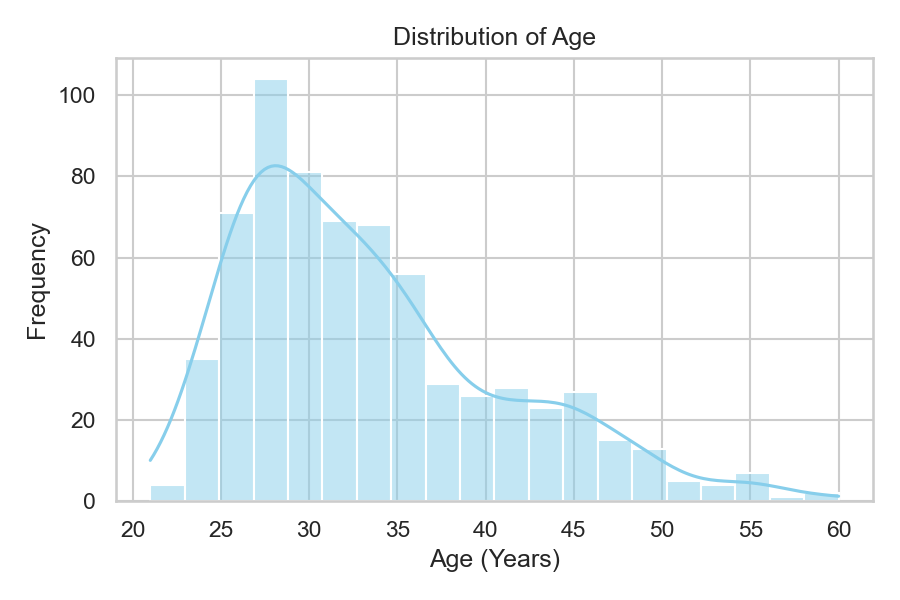
\includegraphics[width=\textwidth]{hist_age.png}
        \caption{Age Distribution}
    \end{minipage}\hfill
    \begin{minipage}{0.32\textwidth}
        \centering
        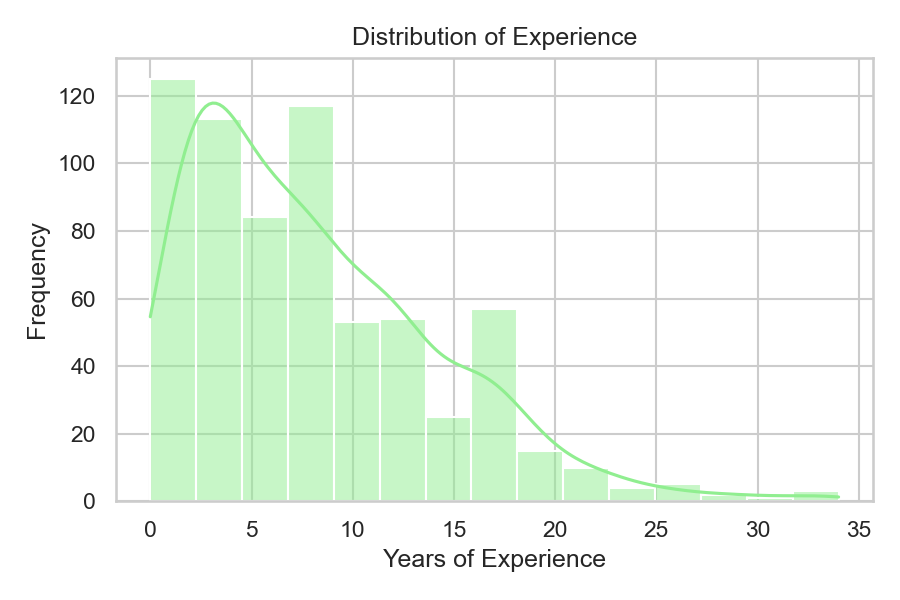
\includegraphics[width=\textwidth]{hist_experience.png}
        \caption{Experience Distribution}
    \end{minipage}\hfill
    \begin{minipage}{0.32\textwidth}
        \centering
        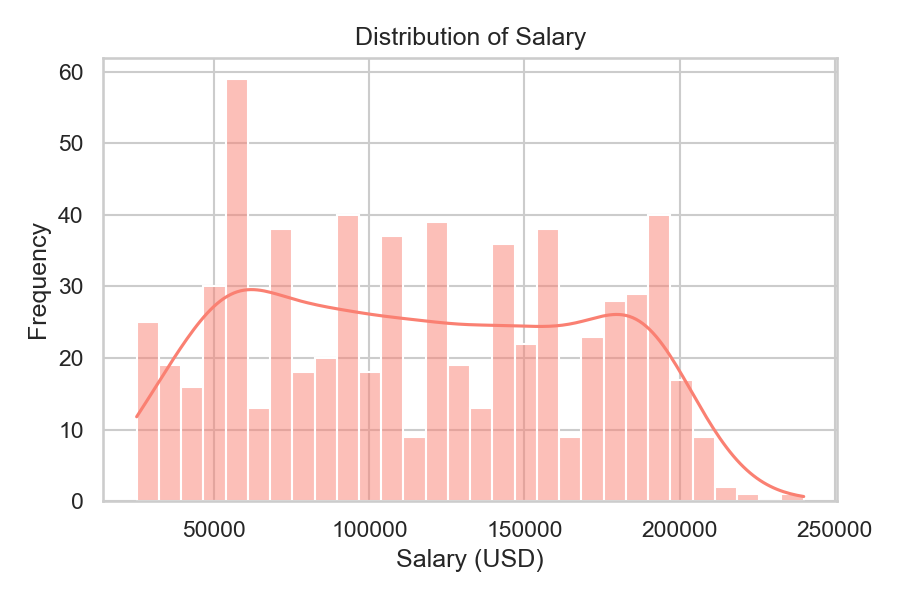
\includegraphics[width=\textwidth]{hist_salary.png}
        \caption{Salary Distribution}
    \end{minipage}
\end{figure}

The histogram for Age suggests a mildly right-skewed distribution, with the sample concentrated among relatively younger employees. Professional experience also appears right-skewed, with a noticeable concentration at lower values. These descriptive patterns make a non-linear specification for experience plausible, although the case for including higher-order terms should be evaluated primarily through model fit and coefficient diagnostics rather than from the histogram alone. Finally, the Salary distribution appears dispersed and right-skewed. This descriptive evidence supports considering the logarithmic transformation (\(\ln(\text{Salary})\)) in Models 2 and 3 to improve interpretability and potentially reduce distributional asymmetry.

\subsection{Correlation Analysis}
Table~\ref{tab:corr} reports the correlation matrix among the variables.

A strong positive correlation is observed between Age and Years of Experience (0.939), which is expected, as older individuals typically have accumulated more work experience. However, this high correlation also suggests the potential presence of multicollinearity, which will be further examined in the diagnostics section.

Salary is positively correlated with both Age (0.720) and Years of Experience (0.791), indicating that income tends to increase with both age and work experience. Notably, the correlation between Salary and Years of Experience is stronger, suggesting that experience may be a more important determinant of earnings than age.

The logarithm of salary (\(\ln(\text{Salary})\)) also shows strong positive correlations with Salary (0.909), Years of Experience (0.696), and Age (0.624). The high correlation between Salary and \(\ln(\text{Salary})\) indicates that the transformation preserves the broad ranking of observations while potentially offering a more convenient functional form for regression analysis.

\begin{table}[htpb]
\centering
\caption{Correlation Matrix}
\label{tab:corr}
\begin{tabular}{lrrrr}
\toprule
& \textbf{Age} & \textbf{Experience} & \textbf{Salary} & \textbf{\(\ln(\text{Salary})\)} \\
\midrule
Age & 1.000 & & & \\
Experience & \textbf{0.939} & 1.000 & & \\
Salary & 0.720 & 0.791 & 1.000 & \\
\(\ln(\text{Salary})\) & 0.624 & 0.696 & 0.909 & 1.000 \\
\bottomrule
\end{tabular}
\end{table}

\subsection{Preliminary Insights}
From the descriptive statistics and correlation analysis, several important insights can be drawn.
First, salary exhibits a high level of variability, indicating heterogeneity among individuals in the dataset. Second, Years of Experience appears to have a stronger relationship with salary compared to age, suggesting it may play a more significant role in explaining income differences. Finally, the strong correlation between Age and Years of Experience raises concerns about multicollinearity, which may affect the stability of regression estimates.

% ══════════════════════════════════════════════════════════════════════════════
\section{Model Estimation and Results}

\subsection{Model Specification}
Three Ordinary Least Squares (OLS) models are estimated to examine the determinants of salary.
Model~1 uses salary in levels as the dependent variable.
Model~2 applies a logarithmic transformation of salary (\(\ln(\text{Salary})\)) to address potential skewness and heteroskedasticity.
Model~3 extends Model~2 by incorporating nonlinear effects of age and interaction terms between experience and education.

\subsection{Estimation Results}
Table~\ref{tab:regression} presents the regression results for all three models.

\begin{table}[htpb]
\centering
\caption{Regression Results Comparison}
\label{tab:regression}
\resizebox{\textwidth}{!}{
\begin{tabular}{lrrr}
\toprule
& \textbf{Model 1} & \textbf{Model 2} & \textbf{Model 3} \\
& \textit{(Level-Level)} & \textit{(Log-Level)} & \textit{(Log-Level Extended)} \\
\midrule
\textbf{Intercept} & 63,493.00*** & 10.719*** & 10.264*** \\
\textbf{Age} & $-$1,593.65** & $-$0.0158*** & --- \\
\textbf{Age\_c} & --- & --- & $-$0.0078 \\
\textbf{Age2\_c} & --- & --- & $-$0.0009*** \\
\textbf{Experience} & 7,182.80*** & 0.0691*** & 0.0827*** \\
\textbf{Male} & 5,602.15. & 0.0629** & 0.0549. \\
\textbf{Other} & $-$26,771.07 & 0.1073 & $-$0.1600 \\
\textbf{Bachelor} & 36,908.32*** & 0.6943*** & 0.6185*** \\
\textbf{Master} & 48,751.38*** & 0.8468*** & 0.8575*** \\
\textbf{PhD} & 57,442.79*** & 0.8554*** & 1.0627*** \\
\textbf{Exp \(\times\) Bachelor} & --- & --- & $-$0.0034 \\
\textbf{Exp \(\times\) Master} & --- & --- & $-$0.0199*** \\
\textbf{Exp \(\times\) PhD} & --- & --- & $-$0.0291*** \\
\midrule
\textbf{\(R^2\)} & 0.6968 & 0.7133 & 0.7485 \\
\textbf{Adj. \(R^2\)} & 0.6917 & 0.7085 & 0.7418 \\
\textbf{AIC} & 9,957.4 & 189.2 & 141.6 \\
\textbf{N} & 425 & 425 & 425 \\
\bottomrule
\end{tabular}
}
\\[1ex]
\textit{\small Note: *** \(p<0.001\), ** \(p<0.01\), * \(p<0.05\), . \(p<0.1\). Standard Errors are HC3 robust. Base: Female, High School.}
\end{table}

\textbf{Model 1 (Level--Level Model)}\\
In Model 1, salary is regressed on age, years of experience, gender, and education.
Years of experience has a positive and statistically significant association with salary. In Model 1, one additional year of experience is associated with an increase of approximately 7,183 salary units, holding the other regressors constant ($p < 0.001$).
Age, however, has a negative and statistically significant coefficient ($-1,593$), suggesting that after controlling for experience and the other included covariates, older individuals in this sample tend to earn slightly less on average. Given the high correlation between age and experience, this coefficient should be interpreted cautiously.
Education is strongly associated with income in the estimated model. Compared with individuals whose highest education is high school:
\begin{itemize}
  \item A bachelor's degree increases salary by about \$36,908
  \item A master's degree increases salary by about \$48,751
  \item A PhD increases salary by about \$57,443
\end{itemize}
All education variables are highly significant ($p < 0.001$).
Gender differences are less pronounced. Male workers earn approximately \$5,602 more than females, but this effect is only marginally significant ($p \approx 0.059$).

\vspace{1em}
\textbf{Model 2 (Log--Level Model)}\\
Model 2 uses the logarithm of salary as the dependent variable, so coefficients on continuous regressors are interpreted approximately as semi-elasticities.
Years of experience remains highly significant, with a coefficient of 0.069. This implies that each additional year of experience is associated with an increase in salary of approximately 6.9\%, holding other factors constant.
Education continues to show a strong positive association with salary. Applying the exact semi-elasticity formula $\left(e^{\hat{\beta}} - 1\right) \times 100\%$ to the dummy variable coefficients yields:
\begin{itemize}
  \item Bachelor's degree: $e^{0.6943} - 1 \approx +100.2\%$
  \item Master's degree: $e^{0.8468} - 1 \approx +132.9\%$
  \item PhD: $e^{0.8554} - 1 \approx +135.2\%$
\end{itemize}
All education effects are statistically significant at the 1\% level.
Age has a small but statistically significant negative coefficient ($-0.0158$), indicating that a one-year increase in age is associated with roughly 1.6\% lower salary, conditional on experience and the other included regressors.
Gender becomes statistically significant in this model. The coefficient on the male indicator implies that male employees have salaries that are approximately 6.5\% higher than those of female employees, using the exact transformation $\exp(0.0629)-1$, with $p < 0.05$.

\vspace{1em}
\textbf{Model 3 (Extended Log Model)}\\
Model 3 introduces nonlinear age effects and interaction terms.
The squared age term (\(\text{Age}_c^2\)) is negative and statistically significant, indicating a concave relationship between age and log salary within this specification. Although the linear term $\text{Age}_c$ is not individually significant, a joint F-test for $H_0\!: \beta_{\text{Age}_c} = \beta_{\text{Age}_c^2} = 0$ yields $F(2, 413) = 10.30$ ($p < 0.001$), confirming that the age polynomial jointly contributes significant explanatory power. The age profile should therefore be interpreted based on the joint test rather than the individual coefficient alone.
Years of experience remains strongly positive and significant (approximately 8.27\% per additional year for the baseline education group).
The interaction terms suggest that:
\begin{itemize}
  \item The return to experience is lower for individuals with higher education levels
  \item This effect is significant for Master's and PhD degrees ($\hat{\delta}_{\text{Master}} = -0.0199$, $\hat{\delta}_{\text{PhD}} = -0.0291$)
\end{itemize}
These coefficients are negative and statistically significant, which is \textbf{contrary to the direction predicted by H4} (which expected $\hat{\delta}_j > 0$). H4 is therefore \textbf{rejected}. The estimated marginal returns to experience for the baseline (High School) group are approximately 8.27\% per year; for Master's holders they are $0.0827 - 0.0199 \approx 6.3\%$, and for PhD holders $0.0827 - 0.0291 \approx 5.4\%$. All returns remain positive and economically meaningful --- the result is not a ``ceiling'' but rather \textbf{diminishing marginal returns to experience by education level}. A straightforward mechanical explanation suffices: highly educated workers command higher starting salaries, so the same absolute annual increment represents a smaller percentage gain, producing a lower experience slope without implying any salary ceiling.

\subsection{Model Comparison}
Table~\ref{tab:model_compare} summarises the in-sample fit criteria for all three models.

\begin{table}[htpb]
\centering
\caption{Model Comparison: Goodness-of-Fit Criteria}
\label{tab:model_compare}
\begin{tabular}{lrrrr}
\toprule
& \textbf{Model 1} & \textbf{Model 2} & \textbf{Model 3} \\
\midrule
$R^2$ & 0.697 & 0.713 & 0.748 \\
Adj.\ $R^2$ & 0.692 & 0.709 & 0.742 \\
AIC & 9{,}957.4 & 189.2 & 141.6 \\
BIC & 9{,}989.8 & 221.6 & 190.3 \\
$N$ & 425 & 425 & 425 \\
\bottomrule
\end{tabular}
\end{table}

A formal \textbf{F-test for nested model comparison} (Model~2 vs.\ Model~3) tests whether the four additional terms introduced in Model~3 ($\text{Age}_c^2$ and three education--experience interactions) jointly contribute explanatory power. The test statistic is:
\[
  F(4,\,413) = 14.42, \quad p < 0.001
\]
The null hypothesis that all added coefficients are jointly zero is strongly rejected, confirming that Model~3 provides a statistically significant improvement in fit over Model~2. Nevertheless, this formal improvement must be balanced against the substantially higher multicollinearity (VIF $> 20$ for several terms) and reduced interpretability of the extended specification. Model~2 is therefore retained as the \textbf{preferred reporting model}, with Model~3 serving as an extended robustness check.

\subsection{Key Findings}
Several important conclusions emerge from the regression analysis.
First, years of experience is the most consistently significant covariate across all models.
Second, education is strongly associated with higher earnings, with larger estimated coefficients for higher attainment levels relative to the High School base group.
Third, gender differences are present but smaller in magnitude than the estimated effects of experience and education.
Finally, Model 3 suggests that the relationship between age and salary may be non-linear and that the return to experience may vary across education groups.

% ══════════════════════════════════════════════════════════════════════════════
\section{Model Diagnostics}

\subsection{Multicollinearity (VIF Test)}
The Variance Inflation Factor (VIF) is used to detect multicollinearity among explanatory variables.
For Model 1 and Model 2, the VIF values for Age and Years of Experience are approximately 8.7--8.8, indicating a relatively high correlation between these variables. This is consistent with the earlier correlation analysis and suggests moderate multicollinearity, although the values remain below the common threshold of 10.
Education variables exhibit moderate VIF values (around 3.7--3.8), which do not raise serious concerns. Gender variables have very low VIF values (close to 1), indicating no multicollinearity issues.
For Model 3, the inclusion of interaction terms significantly increases multicollinearity. Some variables, such as Exp \(\times\) PhD and Years of Experience, have very high VIF values (above 20), indicating strong multicollinearity. This is expected due to the inclusion of interaction terms and polynomial transformations.
Overall, while multicollinearity is present---especially in Model 3---it is not unexpected given the model specification and does not invalidate the results, though it may reduce the precision of some coefficient estimates.

\begin{table}[htpb]
\centering
\caption{Variance Inflation Factor (VIF)}
\label{tab:vif}
\begin{tabular}{lrrr}
\toprule
\textbf{Variable} & \textbf{Model 1} & \textbf{Model 2} & \textbf{Model 3} \\
\midrule
Age / Age\_c & 8.69 & 8.69 & 9.22 \\
Experience & 8.80 & 8.80 & 24.21 \\
Age2\_c & --- & --- & 2.38 \\
Exp \(\times\) PhD & --- & --- & 27.95 \\
Exp \(\times\) Master & --- & --- & 14.98 \\
Exp \(\times\) Bachelor & --- & --- & 9.93 \\
\bottomrule
\end{tabular}
\end{table}

\subsection{Heteroskedasticity (Breusch--Pagan Test)}
The Breusch--Pagan test \citep{breusch1979} is conducted to examine whether the variance of the residuals is constant.
The results indicate that heteroskedasticity is present in all three models. The p-values for the test are extremely small ($p < 0.001$), leading to rejection of the null hypothesis of homoskedasticity.
This implies that the variance of the error term is not constant, which may leave OLS coefficient estimates unbiased under the usual exogeneity condition but makes the conventional homoskedastic standard errors unreliable.

As a correction strategy, HC3 heteroskedasticity-robust standard errors are applied rather than Weighted Least Squares (WLS). This choice is deliberate: WLS requires a correctly specified variance function $\text{Var}(u_i | \mathbf{x}_i) = \sigma^2 h(\mathbf{x}_i)$ which is not known a priori in this setting. Misspecifying the weights in WLS can introduce bias that may exceed the efficiency gains it provides \citep{wooldridge2010}. HC3 robust inference, by contrast, remains valid without assuming a particular form of heteroskedasticity. Table~\ref{tab:se_compare} illustrates the impact on the standard errors of Model~1.

\textbf{Note on the ``Other'' gender category:} A single observation ($n = 1$) in the ``Other'' gender group generates a near-singular sub-matrix, which is why the HC3 standard error for this coefficient in Model~2 is extremely large (SE $= 58.857$). This coefficient is effectively uninformative and should not be used for inference. In a larger sample, this group would either be adequately represented or merged with a reference category.

\begin{table}[htpb]
\centering
\caption{Comparison of Standard Errors for Model 1 (Level-Level)}
\label{tab:se_compare}
\begin{tabular}{lrrr}
\toprule
\textbf{Variable} & \textbf{Non-robust SE} & \textbf{HC3 Robust SE} & \textbf{\% Change} \\
\midrule
Intercept & 14,342.24 & 15,644.48 & +9.08\% \\
Age & 541.90 & 629.42 & +16.15\% \\
Experience & 650.24 & 837.38 & +28.78\% \\
Male & 2,887.00 & 2,957.30 & +2.44\% \\
Bachelor & 5,623.27 & 2,924.89 & $-$47.99\% \\
Master & 6,025.93 & 3,897.07 & $-$35.33\% \\
PhD & 6,876.17 & 5,206.16 & $-$24.29\% \\
\bottomrule
\end{tabular}
\end{table}

\begin{figure}[htpb]
    \centering
    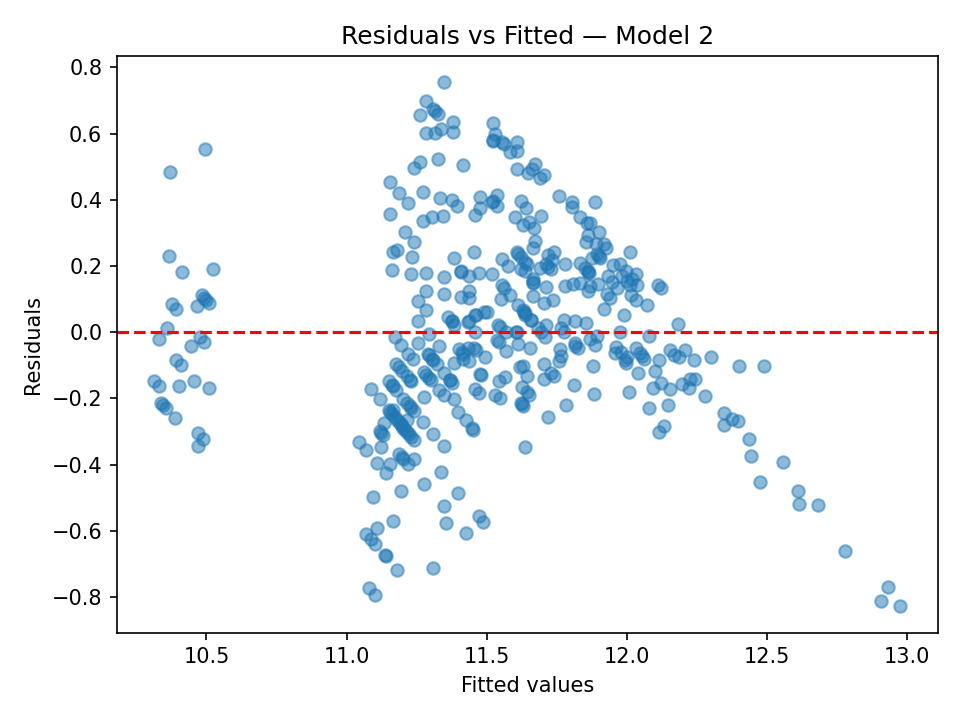
\includegraphics[width=0.6\textwidth]{resid_vs_fitted_model2.png}
    \caption{Residuals vs Fitted Values for Model 2}
    \label{fig:resid_fitted}
\end{figure}

\begin{table}[htpb]
\centering
\caption{Breusch--Pagan Test for Heteroskedasticity}
\label{tab:bp}
\begin{tabular}{lrrl}
\toprule
\textbf{Model} & \textbf{LM stat} & \textbf{p-value} & \textbf{Conclusion} \\
\midrule
Model 1 & 46.82 & $< 0.001$ & Heteroskedasticity present \\
Model 2 & 47.16 & $< 0.001$ & Heteroskedasticity present \\
Model 3 & 83.88 & $< 0.001$ & Heteroskedasticity present \\
\bottomrule
\end{tabular}
\end{table}

\subsection{Normality of Residuals (Jarque--Bera Test)}
The Jarque--Bera test \citep{jarque1980} is used to assess whether the residuals follow a normal distribution.
For Model 1, the null hypothesis of normality is rejected ($p < 0.01$), indicating that the residuals are not normally distributed.
For Model 2, the p-value is high ($p \approx 0.91$), so the null hypothesis of normality is not rejected. This is consistent with the view that the log transformation improves the residual distribution in this specification.
For Model 3, the null hypothesis is rejected again ($p \approx 0.012$), indicating deviations from normality.

\begin{figure}[htpb]
    \centering
    \begin{minipage}{0.32\textwidth}
        \centering
        
\includegraphics[width=\textwidth]{qqplot_model1_level_level.png}
        \caption{QQ-Plot (Model 1)}
    \end{minipage}\hfill
    \begin{minipage}{0.32\textwidth}
        \centering
        
\includegraphics[width=\textwidth]{qqplot_model2_log_level.png}
        \caption{QQ-Plot (Model 2)}
    \end{minipage}\hfill
    \begin{minipage}{0.32\textwidth}
        \centering
        
\includegraphics[width=\textwidth]{qqplot_model3_log_level_extended.png}
        \caption{QQ-Plot (Model 3)}
    \end{minipage}
    \vspace{0.5em}
    
    \textit{\small Note: With a sample size of $n = 425$, mild violations of normality (as seen in Models 1 and 3) are generally not a major issue due to the Central Limit Theorem.}
\end{figure}

\begin{table}[htpb]
\centering
\caption{Jarque--Bera Test for Normality}
\label{tab:jb}
\begin{tabular}{lrrrrl}
\toprule
\textbf{Model} & \textbf{JB stat} & \textbf{p-value} & \textbf{Skew} & \textbf{Kurtosis} & \textbf{Conclusion} \\
\midrule
Model 1 & 24.98 & $< 0.001$ & 0.583 & 3.224 & Reject normality \\
Model 2 & 0.18 & 0.912 & $-0.040$ & 3.062 & Fail to reject \\
Model 3 & 8.82 & 0.012 & 0.338 & 3.199 & Reject normality \\
\bottomrule
\end{tabular}
\end{table}

\subsection{Overall Assessment}
Based on the diagnostic tests, several conclusions can be drawn.
First, multicollinearity exists, particularly between Age and Years of Experience, and becomes more severe in the extended model due to interaction terms.
Second, heteroskedasticity is present in all models, making the use of robust standard errors necessary for reliable inference.
Third, Model 2 performs best in terms of residual normality among the three specifications, which is consistent with using the log transformation of salary.

\subsection{Preferred Model}
Considering model fit, interpretability, and diagnostic results, Model 2 (log-level model) is preferred as the main specification.
Although Model 3 has a better in-sample fit (higher $R^2$ and lower AIC and BIC relative to Model~2, as shown in Table~\ref{tab:model_compare}), it also suffers from stronger multicollinearity and is harder to interpret. In contrast, Model 2 provides a more balanced specification for reporting the core results, while Model 3 can be treated as an extended robustness check.

The Durbin--Watson statistic reported for Model~2 is $DW = 1.748$, which is close to 2 and indicates no evidence of first-order serial correlation in the residuals. Since this study uses cross-sectional data, where observations have no natural ordering in time, serial autocorrelation is not a theoretical concern; the Durbin--Watson statistic is reported here for completeness only.

% ══════════════════════════════════════════════════════════════════════════════
\section{Conclusions, Comments and Recommendations}
% ══════════════════════════════════════════════════════════════════════════════

\subsection{Summary of Findings}
This study examined the determinants of individual salary using a cross-sectional dataset of $n = 425$ employees, estimating three nested OLS models. Evaluating the four research hypotheses against the empirical results:

\textbf{H1 (Returns to Experience) --- Supported.} Years of experience is positively and significantly associated with salary across all three models (e.g., Model~2: $\hat{\beta} = 0.069$, $p < 0.001$). Each additional year of experience is associated with approximately 6.9\% higher salary, consistent with human capital theory.

\textbf{H2 (Education Premium) --- Supported, with qualification.} All three higher education levels yield significantly higher salaries than the High School baseline, with estimated premia of Bachelor's (+100.2\%), Master's (+132.9\%), and PhD (+135.2\%). The ordering is consistent with human capital theory. However, the 95\% confidence intervals for Master's ($[0.737,\,0.956]$) and PhD ($[0.729,\,0.981]$) overlap substantially, and the difference between these two coefficients ($\Delta = 0.0086$) is not statistically distinguishable. H2 is therefore supported for the High School--Bachelor--Master ordering, but the Master--PhD premium cannot be ranked with statistical confidence.

\textbf{H3 (Non-Linear Age Effects) --- Partially Supported.} H3 requires both a positive $\hat{\beta}_{\text{Age}_c}$ (rising returns in early career) and a negative $\hat{\beta}_{\text{Age}_c^2}$ (diminishing returns at later stages). The squared term is negative and significant ($\hat{\beta} = -0.0009$, $p < 0.001$), confirming diminishing returns with age. However, the linear term $\text{Age}_c$ is not statistically significant ($\hat{\beta} = -0.0078$, $p > 0.05$), so the positive early-career portion of the inverted U-shape cannot be confirmed from the data. H3 is therefore only \textbf{partially supported}: the concave curvature is confirmed but the full inverted U-shape is not.

\textbf{H4 (Conditional Returns to Experience) --- Rejected.} Contrary to prediction, the interaction terms for Master's and PhD education are negative and significant, indicating \textbf{diminishing marginal returns to experience by education level}. PhD holders earn approximately 5.4\% per additional year of experience (vs.\ 8.3\% for the High School baseline), and Master's holders earn approximately 6.3\%. Returns remain positive across all groups; the result reflects a lower slope, not a salary ceiling.

\subsection{Comments on Methodology}
The preferred specification (Model~2) satisfies the OLS normality assumption (Jarque--Bera, $p = 0.912$), while heteroskedasticity is corrected through HC3 robust standard errors. Multicollinearity between Age and Experience is addressed via mean-centring in Model~3 rather than variable exclusion, preserving theoretical completeness at the cost of higher VIF values in the extended specification. The single-observation ``Other'' gender category produces an uninformative coefficient with excessively large standard error and should be interpreted with caution.

\subsection{Recommendations}
\textbf{For individuals:} Investing in postgraduate education yields substantial earnings premiums. Given that the return to experience is relatively stronger for lower-educated workers, individuals without postgraduate degrees benefit disproportionately from accumulating years of professional experience early in their careers.

\textbf{For employers and HR practitioners:} Compensation structures should recognise the significant education premium and the diminishing marginal return to experience for highly educated workers. Performance-linked remuneration may better align incentives for senior, highly-educated employees than purely tenure-based pay systems.

\textbf{For policymakers:} The persistent gender wage gap after controlling for observable human capital factors suggests the presence of structural or institutional barriers. Wage transparency legislation and equality audits represent evidence-based policy tools to address this residual gap.

\subsection{Limitations and Future Research}
This study is limited by its cross-sectional design, which precludes causal identification of experience returns; by the absence of controls for industry, occupation, and firm size; and by the relatively small sample ($n = 425$). Future work should employ panel data to separate cohort effects from genuine experience returns, and should incorporate a richer set of controls to reduce omitted variable bias.

% ══════════════════════════════════════════════════════════════════════════════
% References
% ══════════════════════════════════════════════════════════════════════════════
\newpage
\bibliographystyle{apalike}

% ── Inline bibliography (no .bib file needed) ──────────────────────────────────
\begin{thebibliography}{99}

\bibitem[Becker(1964)]{becker1964}
Becker, G.~S. (1964).
\newblock \textit{Human Capital: A Theoretical and Empirical Analysis, with
  Special Reference to Education}.
\newblock University of Chicago Press.

\bibitem[Ben-Porath(1967)]{benporath1967}
Ben-Porath, Y. (1967).
\newblock The production of human capital and the life cycle of earnings.
\newblock \textit{Journal of Political Economy}, 75(4), 352--365.

\bibitem[Blau \& Kahn(2017)]{blaukahn2017}
Blau, F.~D. and Kahn, L.~M. (2017).
\newblock The gender wage gap: Extent, trends, and explanations.
\newblock \textit{Journal of Economic Literature}, 55(3), 789--865.

\bibitem[Breusch \& Pagan(1979)]{breusch1979}
Breusch, T.~S. and Pagan, A.~R. (1979).
\newblock A simple test for heteroscedasticity and random coefficient variation.
\newblock \textit{Econometrica}, 47(5), 1287--1294.

\bibitem[Card(1999)]{card1999}
Card, D. (1999).
\newblock The causal effect of education on earnings.
\newblock In O.~Ashenfelter and D.~Card (Eds.), \textit{Handbook of Labor
  Economics}, Vol.~3A, pp.\ 1801--1863. Elsevier.

\bibitem[Jarque \& Bera(1980)]{jarque1980}
Jarque, C.~M. and Bera, A.~K. (1980).
\newblock Efficient tests for normality, homoscedasticity and serial independence of regression residuals.
\newblock \textit{Economics Letters}, 6(3), 255--259.

\bibitem[Lemieux(2006)]{lemieux2006}
Lemieux, T. (2006).
\newblock The Mincer equation thirty years after \textit{Schooling, Experience
  and Earnings}.
\newblock In S.~Grossbard (Ed.), \textit{Jacob Mincer: A Pioneer of Modern
  Labor Economics}. Springer.

\bibitem[Mincer(1974)]{mincer1974}
Mincer, J. (1974).
\newblock \textit{Schooling, Experience and Earnings}.
\newblock National Bureau of Economic Research.

\bibitem[Spence(1973)]{spence1973}
Spence, M. (1973).
\newblock Job market signalling.
\newblock \textit{Quarterly Journal of Economics}, 87(3), 355--374.

\bibitem[Wooldridge(2010)]{wooldridge2010}
Wooldridge, J.~M. (2010).
\newblock \textit{Econometric Analysis of Cross Section and Panel Data} (2nd
  ed.).
\newblock MIT Press.

\end{thebibliography}

% ══════════════════════════════════════════════════════════════════════════════
\newpage
\appendix
\section{Supplementary Materials}
\label{app:supp}

\subsection{Appendix A: Model 1 (Linear) Summary Output}

\noindent\textbf{SUMMARY OUTPUT}\\[0.4em]
\textit{Dependent variable: Salary (USD). Base categories: Female, High School. HC3 robust standard errors.}

\begin{table}[H]
\centering\scriptsize
\caption*{\textit{Regression Statistics — Model 1}}
\begin{tabular}{lr}
\toprule
Multiple R & 0.8347 \\
R Square & 0.6968 \\
Adjusted R Square & 0.6917 \\
Standard Error & 29{,}328.15 \\
Observations & 425 \\
\bottomrule
\end{tabular}
\end{table}

\begin{table}[H]
\centering\scriptsize
\caption*{\textit{ANOVA — Model 1}}
\begin{tabular}{lrrrrr}
\toprule
 & \textbf{df} & \textbf{SS} & \textbf{MS} & \textbf{F} & \textbf{Significance F} \\
\midrule
Regression & 7 & 824,120,516,974.71 & 117,731,502,424.96 & 136.87 & 0.0000 \\
Residual   & 417 & 358,678,489,624.50 & 860,140,262.89 & & \\
Total      & 424 & 1,182,799,006,599.21 & & & \\
\bottomrule
\end{tabular}
\end{table}

\begin{table}[H]
\centering\scriptsize
\caption*{\textit{Coefficients — Model 1}}
\begin{tabular}{lrrrrrr}
\toprule
\textbf{Variable} & \textbf{Coeff.} & \textbf{Std Error} & \textbf{t Stat} & \textbf{P-value} & \textbf{Lower 95\%} & \textbf{Upper 95\%} \\
\midrule
Intercept          & 63,493.00 & 15,644.48 & 4.0585 & 0.0001 & 32,741.13 & 94,244.87 \\
Gender (Male)      &  5,602.15 &  2,957.30 & 1.8943 & 0.0589 &   -210.92 & 11,415.21 \\
Gender (Other)     & -26,771.07 & 355,923.37 & -0.0752 & 0.9401 & -726,398.66 & 672,856.51 \\
Bachelor           & 36,908.32 &  2,924.89 & 12.6187 & 0.0000 & 31,158.95 & 42,657.69 \\
Master             & 48,751.38 &  3,897.07 & 12.5098 & 0.0000 & 41,091.03 & 56,411.73 \\
PhD                & 57,442.79 &  5,206.16 & 11.0336 & 0.0000 & 47,209.20 & 67,676.38 \\
Age                & -1,593.65 &    629.42 & -2.5319 & 0.0117 & -2,830.88 &   -356.42 \\
Years of Experience &  7,182.80 &    837.38 &  8.5777 & 0.0000 &  5,536.78 &  8,828.81 \\
\bottomrule
\end{tabular}
\end{table}

% ─────────────────────────────────────────────────────────────────────────────
\subsection{Appendix B: Model 2 (Semi-Log) Summary Output}

\noindent\textbf{SUMMARY OUTPUT}\\[0.4em]
\textit{Dependent variable: ln(Salary). Base categories: Female, High School. HC3 robust standard errors.}

\begin{table}[H]
\centering\scriptsize
\caption*{\textit{Regression Statistics — Model 2}}
\begin{tabular}{lr}
\toprule
Multiple R & 0.8446 \\
R Square & 0.7133 \\
Adjusted R Square & 0.7085 \\
Standard Error & 0.2995 \\
Observations & 425 \\
\bottomrule
\end{tabular}
\end{table}

\begin{table}[H]
\centering\scriptsize
\caption*{\textit{ANOVA — Model 2}}
\begin{tabular}{lrrrrr}
\toprule
 & \textbf{df} & \textbf{SS} & \textbf{MS} & \textbf{F} & \textbf{Significance F} \\
\midrule
Regression & 7 & 93.0766 & 13.2967 & 148.2380 & 0.0000 \\
Residual   & 417 & 37.4041 & 0.0897 & & \\
Total      & 424 & 130.4807 & & & \\
\bottomrule
\end{tabular}
\end{table}

\begin{table}[H]
\centering\scriptsize
\caption*{\textit{Coefficients — Model 2}}
\begin{tabular}{lrrrrrr}
\toprule
\textbf{Variable} & \textbf{Coeff.} & \textbf{Std Error} & \textbf{t Stat} & \textbf{P-value} & \textbf{Lower 95\%} & \textbf{Upper 95\%} \\
\midrule
Intercept           & 10.7187 & 0.1532 & 69.9483 & 0.0000 & 10.4175 & 11.0199 \\
Gender (Male)       &  0.0629 & 0.0304 &  2.0725 & 0.0388 &  0.0032 &  0.1226 \\
Gender (Other)      &  0.1073 & 60.0001 &  0.0018 & 0.9986 & -117.8331 & 118.0477 \\
Bachelor            &  0.6943 & 0.0506 & 13.7192 & 0.0000 &  0.5948 &  0.7937 \\
Master              &  0.8468 & 0.0556 & 15.2313 & 0.0000 &  0.7375 &  0.9560 \\
PhD                 &  0.8554 & 0.0641 & 13.3347 & 0.0000 &  0.7293 &  0.9815 \\
Age                 & -0.0158 & 0.0058 & -2.7458 & 0.0063 & -0.0271 & -0.0045 \\
Years of Experience &  0.0691 & 0.0082 &  8.4665 & 0.0000 &  0.0531 &  0.0852 \\
\bottomrule
\end{tabular}
\end{table}

% ─────────────────────────────────────────────────────────────────────────────
\subsection{Appendix C: Model 3 (Quadratic -- Final) Summary Output}

\noindent\textbf{SUMMARY OUTPUT}\\[0.4em]
\textit{Dependent variable: ln(Salary). Base categories: Female, High School. HC3 robust standard errors.}

\begin{table}[H]
\centering\scriptsize
\caption*{\textit{Regression Statistics — Model 3}}
\begin{tabular}{lr}
\toprule
Multiple R & 0.8651 \\
R Square & 0.7485 \\
Adjusted R Square & 0.7418 \\
Standard Error & 0.2819 \\
Observations & 425 \\
\bottomrule
\end{tabular}
\end{table}

\begin{table}[H]
\centering\scriptsize
\caption*{\textit{ANOVA — Model 3}}
\begin{tabular}{lrrrrr}
\toprule
 & \textbf{df} & \textbf{SS} & \textbf{MS} & \textbf{F} & \textbf{Significance F} \\
\midrule
Regression & 11 & 97.6615 &  8.8783 & 111.7255 & 0.0000 \\
Residual   & 413 & 32.8192 &  0.0795 & & \\
Total      & 424 & 130.4807 & & & \\
\bottomrule
\end{tabular}
\end{table}

\begin{table}[H]
\centering\scriptsize
\caption*{\textit{Coefficients — Model 3}}
\begin{tabular}{lrrrrrr}
\toprule
\textbf{Variable} & \textbf{Coeff.} & \textbf{Std Error} & \textbf{t Stat} & \textbf{P-value} & \textbf{Lower 95\%} & \textbf{Upper 95\%} \\
\midrule
Intercept                & 10.2644 & 0.0696 & 147.4113 & 0.0000 & 10.1275 & 10.4013 \\
Gender (Male)            &  0.0549 & 0.0282 &   1.9444 & 0.0525 & -0.0006 &  0.1104 \\
Gender (Other)           & -0.1600 & 48.8535 &  -0.0033 & 0.9974 & -96.1925 & 95.8726 \\
Bachelor                 &  0.6185 & 0.0623 &   9.9331 & 0.0000 &  0.4961 &  0.7409 \\
Master                   &  0.8575 & 0.0792 &  10.8220 & 0.0000 &  0.7017 &  1.0133 \\
PhD                      &  1.0627 & 0.1397 &   7.6068 & 0.0000 &  0.7881 &  1.3373 \\
Age (centred)            & -0.0078 & 0.0066 &  -1.1776 & 0.2396 & -0.0208 &  0.0052 \\
Age$^2$ (centred)        & -0.0009 & 0.0003 &  -2.6405 & 0.0086 & -0.0016 & -0.0002 \\
Years of Experience      &  0.0827 & 0.0073 &  11.3256 & 0.0000 &  0.0683 &  0.0970 \\
Bachelor $\times$ Exp    & -0.0034 & 0.0081 &  -0.4204 & 0.6744 & -0.0194 &  0.0126 \\
Master $\times$ Exp      & -0.0199 & 0.0067 &  -2.9604 & 0.0032 & -0.0331 & -0.0067 \\
PhD $\times$ Exp         & -0.0291 & 0.0093 &  -3.1427 & 0.0018 & -0.0474 & -0.0109 \\
\bottomrule
\end{tabular}
\end{table}


\subsection{Appendix D: Outlier Report (Filtered)}
\begin{table}[htpb]
\centering
\scriptsize
\caption{Hybrid Outlier Removed from Analysis}
\begin{tabular}{rrrrrrrrr}
\toprule
\textbf{row\_id} & \textbf{Salary} & \textbf{Lower} & \textbf{Upper} & \textbf{MZ log} & \textbf{IQR} & \textbf{Log MZ} & \textbf{Hybrid} & \textbf{Kept} \\
\midrule
29 & 350 & -65000.0 & 295000.0 & -9.6301 & False & True & True & False \\
\bottomrule
\end{tabular}
\end{table}

\subsection{Appendix E: Python Source Code (Data Cleaning Pipeline)}
The full analysis pipeline --- including descriptive statistics, visualisations, and diagnostic tests --- is available at:

\begin{center}
  \texttt{\url{https://github.com/mhan0505/Project}}
\end{center}

The core scripts are \texttt{part1\_data\_cleaning.py} (cleaning), \texttt{part3\_ols\_models.py} (estimation), and \texttt{part4\_diagnostics.py} (BP, JB, VIF tests). The two key scripts are reproduced below for self-contained reference.

The following script reads the raw dataset \texttt{Group13\_DSEB66A.xlsx} (submitted separately),
removes 4 exact duplicate rows, standardises education level labels, adds derived columns
(\texttt{lnSalary}, \texttt{Age2}, interaction dummies), and writes the cleaned file
\texttt{Group13\_DSEB66A\_part1\_cleaned.xlsx} used in all subsequent analyses.
\begin{lstlisting}[language=Python,basicstyle=\ttfamily\scriptsize,breaklines=true]
import numpy as np
import pandas as pd

EDUCATION_MAP = {
    "bachelor's degree": "Bachelor", "bachelor's": "Bachelor",
    "master's degree": "Master",    "master's": "Master",
    "phd": "PhD",                   "high school": "High School",
}

def normalize_education(value):
    key = str(value).strip().lower().replace("'", "'").replace("'", "'")
    if key in EDUCATION_MAP:
        return EDUCATION_MAP[key]
    raise ValueError(f"Unexpected education value: {value!r}")

# --- Step 1: Load raw data ---
df = pd.read_excel('Group13_DSEB66A.xlsx')   # raw file submitted with report
print(f"Raw rows: {len(df)}")

# --- Step 2: Drop exact duplicates ---
df = df.drop_duplicates().reset_index(drop=True)
print(f"After dedup: {len(df)}")

# --- Step 3: Standardise education labels ---
df['Education Level'] = df['Education Level'].apply(normalize_education)

# --- Step 4: Derive additional columns ---
df['lnSalary']      = np.log(df['Salary'])
df['Age2']          = df['Age'] ** 2
exp = df['Years of Experience']
df['Exp_x_Bachelor'] = np.where(df['Education Level'] == 'Bachelor', exp, 0.0)
df['Exp_x_Master']   = np.where(df['Education Level'] == 'Master',   exp, 0.0)
df['Exp_x_PhD']      = np.where(df['Education Level'] == 'PhD',      exp, 0.0)

# --- Step 5: Save cleaned file ---
df.to_excel('Group13_DSEB66A_part1_cleaned.xlsx', index=False)
print("Saved: Group13_DSEB66A_part1_cleaned.xlsx")
\end{lstlisting}

\subsection{Appendix F: Python Source Code (OLS Estimation with HC3)}
\begin{lstlisting}[language=Python,basicstyle=\ttfamily\scriptsize,breaklines=true]
import pandas as pd
import numpy as np
import statsmodels.formula.api as smf
from statsmodels.compat.python import lzip

# --- Load cleaned data (n=425): apply hybrid IQR + log-modified z-score outlier rule ---
df = pd.read_excel('Group13_DSEB66A_part1_cleaned.xlsx')
df['log_salary'] = np.log(df['Salary'])
Q1, Q3 = df['Salary'].quantile(0.25), df['Salary'].quantile(0.75)
IQR = Q3 - Q1
lower, upper = Q1 - 1.5*IQR, Q3 + 1.5*IQR
med_log = df['log_salary'].median()
mad_log = (df['log_salary'] - med_log).abs().median()
df['mz_log'] = 0.6745 * (df['log_salary'] - med_log) / mad_log
df['is_iqr_outlier'] = (df['Salary'] < lower) | (df['Salary'] > upper)
df['is_mz_outlier']  = df['mz_log'].abs() > 3.5
df['is_hybrid']      = df['is_iqr_outlier'] | df['is_mz_outlier']
df = df[~df['is_hybrid']].copy()  # n=425 after removing 1 outlier (Salary=350)
df = df.drop(columns=['log_salary', 'mz_log', 'is_iqr_outlier', 'is_mz_outlier', 'is_hybrid'])
df['lnSalary'] = np.log(df['Salary'])
df['Agec'] = df['Age'] - df['Age'].mean()
df['Agec2'] = df['Agec'] ** 2
df.rename(columns={'Years of Experience': 'Experience',
                   'Education Level': 'Education'}, inplace=True)

# --- Model 1: Level-Level ---
m1 = smf.ols('Salary ~ Age + Experience + C(Gender, Treatment(reference="Female"))'
             ' + C(Education, Treatment(reference="High School"))', data=df).fit()
print(m1.get_robustcov_results(cov_type='HC3').summary())

# --- Model 2: Log-Level (Preferred) ---
m2 = smf.ols('lnSalary ~ Age + Experience + C(Gender, Treatment(reference="Female"))'
             ' + C(Education, Treatment(reference="High School"))', data=df).fit()
print(m2.get_robustcov_results(cov_type='HC3').summary())
print(f'AIC: {m2.aic:.2f}  BIC: {m2.bic:.2f}')

# --- Model 3: Log-Level Extended ---
m3 = smf.ols('lnSalary ~ Agec + Agec2 + Experience'
             ' + C(Gender, Treatment(reference="Female"))'
             ' + C(Education, Treatment(reference="High School"))'
             ' + C(Education, Treatment(reference="High School")):Experience',
             data=df).fit()
print(m3.get_robustcov_results(cov_type='HC3').summary())
print(f'AIC: {m3.aic:.2f}  BIC: {m3.bic:.2f}')

# --- F-test: Model 2 vs Model 3 (nested) ---
from scipy import stats
RSS2, RSS3 = sum(m2.resid**2), sum(m3.resid**2)
q = m3.df_model - m2.df_model
F = ((RSS2 - RSS3)/q) / (RSS3/(len(df) - m3.df_model - 1))
p = 1 - stats.f.cdf(F, q, len(df) - m3.df_model - 1)
print(f'F-test M2 vs M3: F({int(q)},{int(len(df)-m3.df_model-1)}) = {F:.4f}, p = {p:.6f}')
\end{lstlisting}

\end{document}
